\chapter{Validation}
\label{chap:validation}

\section{Introduction}

This chapter unfolds as a meticulous exploration into the performance and reliability of the Fair-by-Design workflow. To conduct a thorough assessment, the well known dataset Adult has been strategically chosen as the testing ground. The dataset, rich in socioeconomic and demographic attributes, provides a robust platform for evaluating the workflow's effectiveness across various machine learning algorithms.

The central emphasis of this validation endeavor is to ascertain not only the accuracy and predictive capabilities of the implemented models but also the extent to which the Fair-by-Design workflow succeeds in fostering fairness. The Adult dataset allows for a nuanced examination of how different algorithms respond to the intricacies of real-world data, shedding light on the interplay between accuracy and fairness.

Throughout this chapter, the validation process unfolds systematically, encompassing diverse algorithms applied to the dataset. The goal is to detect both the strengths and potential limitations of the Fair-by-Design approach, providing valuable insights for its application in scenarios where the equitable treatment of individuals and the accuracy of predictions are of paramount importance. The subsequent sections detail the experimental setup, algorithmic choices, and the rigorous evaluation metrics employed to ensure a comprehensive understanding of the Fair-by-Design workflow's performance on the chosen dataset.

\section{Precise Definition of Objectives}
\label{section:val_obj}

In this section, we meticulously outline the objectives that intricately guide the Fair-by-Design workflow, with a primary focus on achieving effective income prediction while concurrently addressing fairness considerations and mitigating biases. The critical components encompass the meticulous identification of protected attributes, the strategic selection of fairness notions, and the corresponding choice of fairness metrics.

\subsection{Prediction Objective}

The overarching objective is to execute a fairness-driven classification task, discerning whether an individual's income exceeds or falls below \$50,000 per year.

\subsection{Protected Attributes}

The identified protected attributes for scrutiny within the Fair-by-Design framework are "Ethnicity" and "Sex." These attributes hold particular significance in the context of potential biases and fairness considerations.

\subsection{Fairness Notions}

To operationalize fairness, two distinct notions are employed, each serving specific objectives:

\begin{itemize}
    \item \emph{Demographic Parity:} The objective is to ensure a consistent distribution of predicted outcomes across different subgroups delineated by the protected attributes. This aligns with the broader goal of fostering equity in predictions.

    \item \emph{Group Fairness:} The goal is to guarantee equitable predictions within specific subgroups defined by protected attributes. This notion emphasizes the need for fairness at a more granular level, considering distinct demographic categories.
\end{itemize}

\subsection{Fairness Metrics}

To quantify and assess fairness in the context of the defined notions, specific fairness metrics are employed:

\begin{itemize}
    \item \emph{For Demographic Parity:} The chosen metric is "Disparate Impact," offering a quantitative measure of the disparate outcomes across different subgroups.

    \item \emph{For Group Fairness:} The metric utilized is "Demographic Parity Difference," providing a nuanced assessment of fairness within specific demographic subgroups.
\end{itemize}

These meticulously defined objectives, coupled with the chosen fairness notions and metrics, collectively establish a robust foundation for the Fair-by-Design workflow. This ensures a focused approach towards accurate predictions while concurrently fostering fairness and equity across diverse subgroups.

\section{Data Collection Details}
\label{section:val_dc}

In this section, we delve into the specifics of the data collection process, providing a comprehensive overview of the dataset and its division into distinct training and test sets.

\subsection{Dataset Overview}

The dataset comprises two distinct sets:

\begin{itemize}
    \item \emph{Training Set:} Consisting of 32,561 items.
    \item \emph{Test Set:} Comprising 16,281 items.
\end{itemize}

\subsection{Dataset Composition}

The dataset encompasses 14 independent features of diverse types, each contributing valuable information for predictive modeling. Additionally, there is one dependent variable, representing whether an individual earns more or less than \$50,000 on an annual basis. Each record within the dataset corresponds to an individual, and the output variable is binary, delineating income categories.

\subsection{Protected Attributes and Encoding Consistency}

As identified in \cref{section:val_obj}, two discrete protected attributes, namely "Ethnicity" and "Sex," play a crucial role in fairness considerations. It is imperative to note that these attributes are discrete in nature. Furthermore, an essential consideration for subsequent analyses pertains to the representation of the output variable. Although it is binary, it is currently encoded as a string. Ensuring consistency in the encoding of this variable across both the training and test sets is of paramount importance for accurate and meaningful analyses in subsequent stages.

This detailed understanding of the dataset's composition and attributes provides a solid foundation for subsequent steps in the Fair-by-Design workflow, facilitating informed decisions regarding model development and fairness considerations.
\section{Data pre-processing}

Starting from the information provided by \cref{section:val_dc} in this section all the variables represend as string as been labeled the same manner. This led to a consistent dataset to be used in the models training.

\section{Algorithm design}
\label{section:val_alg}

In the context of the Fair-by-Design workflow, six key fairness algorithms have been strategically chosen to comprehensively test the workflow's effectiveness. Each algorithm serves a specific purpose within the workflow, contributing to the overarching goal of achieving fairness in predictions.

\subsection{Pre-processing Algorithms}

\subsubsection{Data Augmentation Algorithm}

\begin{itemize}

    \item \emph{Algorithm Description:} The proposed data augmentation algorithm introduces synthetic samples to the training dataset. By augmenting the data, especially focusing on underrepresented groups, the algorithm aims to enhance the model's exposure to diverse scenarios, promoting a more robust understanding of the underlying patterns.

    \item \emph{Reasoning:} Data augmentation is crucial for addressing imbalances in the training data, allowing the model to generalize better across different groups and mitigating biases stemming from insufficient representation.

\end{itemize}

\subsubsection{Fairness Through Unawareness}

\begin{itemize}

    \item \emph{Algorithm Description:} Fairness through unawareness involves deliberately avoiding the use of sensitive attributes in the modeling process. This pre-processing approach aims to promote fairness by excluding potentially biased features, thus reducing the risk of discrimination based on sensitive attributes.

    \item \emph{Reasoning:} Fairness through unawareness is considered to mitigate biases by preventing the model from directly using sensitive attributes, thereby minimizing the potential for biased predictions associated with these attributes.

\end{itemize}

\subsection{In-processing Algorithms}

\subsubsection{ExponentiatedGradient}

\begin{itemize}

    \item \emph{Algorithm Description}: The ExponentiatedGradient algorithm applies iterative re-weighting to the training data, seeking to find a fair classifier by minimizing the disparity in predictions across sensitive groups.

    \item \emph{Reasoning:} ExponentiatedGradient is chosen for its versatility and effectiveness in in-processing fairness. It provides a fine-tuning mechanism during training to achieve parity in predicted outcomes.

\end{itemize}

\subsubsection{GridSearch}

\begin{itemize}

    \item \emph{Algorithm Description:} GridSearch is a generic algorithm that explores a range of hyperparameter values to find the optimal configuration for a fair classifier.

    \item \emph{Reasoning:} GridSearch is included to assess the impact of hyperparameter tuning on fairness outcomes, offering insights into the versatility of the approach.

\end{itemize}

\subsection{Post-processing Algorithms}

\subsubsection{ThresholdOptimizer}

\begin{itemize}

    \item \emph{Algorithm Description:} ThresholdOptimizer focuses on adjusting decision thresholds post-modeling to achieve fairness goals. It provides flexibility in fine-tuning predictions without retraining the entire model.

    \item \emph{Reasoning:} ThresholdOptimizer is included to evaluate the effectiveness of post-processing adjustments in achieving fairness objectives. It offers a practical and interpretable way to balance accuracy and fairness.

\end{itemize}

The choice of these five algorithms is driven by the aim of obtaining a holistic view of the Fair-by-Design workflow's performance. By incorporating diverse pre-processing, in-processing, and post-processing strategies, the evaluation can capture the nuances of fairness considerations at different stages of the machine learning pipeline. This comprehensive approach ensures a thorough exploration of potential biases and fairness enhancements, laying the foundation for a robust and equitable model.

\section{Model training and evaluation}
\label{section:val_mt_eval}

\subsection{Model Training}

\subsubsection{Training Models}

The model training process involves the utilization of two distinct classifiers:

\begin{itemize}

    \item \emph{XGBoost}: XGBoost, an optimized gradient boosting algorithm, is selected for its ability to handle diverse datasets and deliver high predictive accuracy.

    \item \emph{RandomForest Classifier:} RandomForest classifier, known for its ensemble learning approach, is chosen to capture complex relationships in the data and enhance predictive performance.

\end{itemize}


\subsection{Performance Evaluation}

\subsubsection{Results Evaluation}

The evaluation of general results encompasses an assessment of the overall model performance and the computation of fairness metrics.

It's important, before to provide a general view of the results, provide some considerations on the pre-processing algorithms:

\begin{itemize}
    \item \emph{Data augmentation}: this algorithm led the dataset from 32,561 to 261,700.
    \item \emph{Fairness through unawareness}: in order to apply this algorithm the protected attribute have been replaced with their \emph{median} value.
\end{itemize}

In order to provide a tabular representation of the results it's necessary to assign some labels to have a more compressed representation:

\begin{itemize}
    \item \emph{Fairness algorithm}: FairAlg
    \begin{itemize}
        \item \emph{Data augmentation}: DA
        \item \emph{Fairness through unawareness}: FtU
        \item \emph{Exponentiated Gradient}: EG
        \item \emph{GridSearch}: GS
        \item \emph{Threshold Optimizer}: TO
    \end{itemize}
    \item \emph{Model}
    \begin{itemize}
        \item \emph{XGB Classifier}: XGB
        \item \emph{RandomForest Classifier}: RF
    \end{itemize}
    \item \emph{Accuracy}: Acc
    \item \emph{Fairness metric}:
    \begin{itemize}
        \item Protected attribute: Sex
        \begin{itemize}
            \item \emph{Disparate Impact }: DIs
            \item \emph{Demographic Parity Difference}: DPDs
        \end{itemize}
        \item Protected attribute: Race
        \begin{itemize}
            \item \emph{Disparate Impact }: DIr
            \item \emph{Demographic Parity Difference}: DPDr
        \end{itemize}
    \end{itemize}
\end{itemize}

\begin{figure}[H]
    \centering
    \begin{tabular}{|c|c|c|c|c|c|c|}
        \hline
        \textbf{FairAlg} & \textbf{Model} & \textbf{Acc} & \textbf{DIs} & \textbf{DIr} & \textbf{DPDs} & \textbf{DPDr} \\
        \hline
        DA & XGB & 0.7918 & 0.5409 & 0.7352 & 0.0171 & 0.0053 \\
        DA & RF & 0.7890 & 0.5950 & 0.7486 & 0.0155 & 0.0051 \\
        FtU & XGB & 0.8235 & 0.3809 & 0.5703 & 0.0242 & 0.0083 \\
        FtU & RF & 0.8162 & 0.4075 & 0.6308 & 0.0197 & 0.0063 \\
        EG & XGB & 0.8079 & 0.5102 & 0.6802 & 0.0265 & 0.0092 \\
        EG & RF & 0.7949 & 0.6154 & 0.7442 & 0.0174 & 0.0064 \\
        GS & XGB & 0.8086 & 0.4103 & 0.6247 & 0.0149 & 0.0046 \\
        GS & RF & 0.8109 & 0.4325 & 0.6376 & 0.0163 & 0.0052 \\
        TO & XGB & 0.7637 & 0.0000 & 0.0000 & 0.0000 & 0.0000 \\
        TO & RF & 0.7637 & 0.0000 & 0.0000 & 0.0000 & 0.0000 \\
        \hline
    \end{tabular}
    \caption{Models training results}
    \label{fig:results}
\end{figure}

About these results is possible to make some considerations:
\begin{enumerate}
    \item \emph{Threshold Optimizer Performance:} The Threshold Optimizer (TO) algorithm consistently maintains an accuracy of 76.3\%, showcasing a perfect achievement of group fairness while completely lacking in demographic parity. This suggests a trade-off between group fairness and demographic parity, emphasizing the need for careful consideration of the ethical implications associated with eliminating disparate impact.
    
    \item \emph{Discrepancy Between Group Fairness and Demographic Parity:} Across multiple algorithms and models, a consistent pattern emerges where group fairness is approximately better achieved than demographic parity. This divergence highlights the nuanced challenges in simultaneously optimizing for different fairness metrics and calls for a deeper exploration into algorithmic design choices.
    
    \item \emph{Uniform Accuracy Levels:} The accuracy across various scenarios hovers around 80\%, with the post-processing algorithm (TO) showing the minimum accuracy and the XGB model coupled with the Fairness through Unawareness (FtU) algorithm achieving the maximum accuracy. This consistent accuracy level underscores the stability of the Fair-by-Design workflow in maintaining predictive performance while incorporating fairness considerations.
    
    \item \emph{Significance of Fairness through Unawareness (FtU):} The results obtained from the FtU tests are of particular importance as they shed light on concerns raised in the literature, specifically those related to proxy attributes potentially leading to protected ones. The FtU algorithm, paired with the XGB model, demonstrates competitive accuracy and fairness outcomes, emphasizing its role in addressing challenges associated with biased features and mitigating the risk of discrimination.
\end{enumerate}

For each fairness algorithm employed in the Fair-by-Design workflow, the minimum and maximum accuracy values are presented. This analysis provides insights into the range of accuracy outcomes associated with each fairness algorithm.
In order to report a more compact visualization of the results to each algorithm is assigned a numerical identifier:

\begin{figure}[H]
    \centering
    \begin{tabular}{|c|c|}
        \hline
        \textbf{Algorithm} & \textbf{Code} \\
        \hline
        DA & 1 \\
        \hline
        FTU & 2 \\
        \hline
        GS & 3 \\
        \hline
        EG & 4 \\
        \hline
        TO & 5 \\
        \hline
    \end{tabular}
    \caption{Algorithm encoding}
\end{figure}

\paragraph{Accuracy}
\begin{figure}[H]
    \centering
    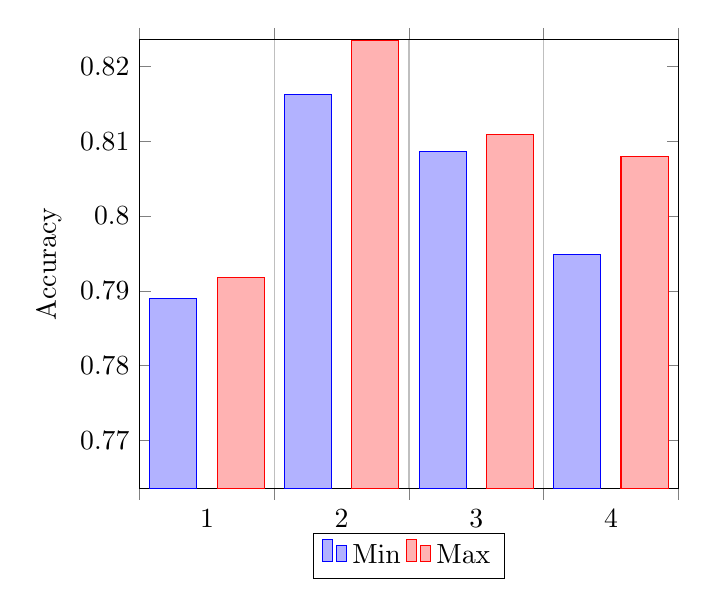
\begin{tikzpicture}
        \begin{axis}[
            x tick label style={
                /pgf/number format/1000 sep=},
            ylabel=Accuracy,
            enlargelimits=0.001,
            legend style={at={(0.5,-0.1)},
            anchor=north,legend columns=-1},
            ybar interval=0.7,
        ]
        \addplot 
            coordinates {(1, 0.7890) (2, 0.8162) (3, 0.8086) (4, 0.7949) (5, 0.7637)};
        \addplot 
            coordinates {(1, 0.7918) (2, 0.8235) (3, 0.8109) (4, 0.8079) (5, 0.7637)};
        \legend{Min,Max}
        \end{axis}
        \end{tikzpicture}
    \caption{Min-Max accuracy for each fairness algorithm}
\end{figure}

There are some considerations that can be made about the accurencies presented:
\begin{enumerate}
    \item \emph{Threshold Optimizer (TO) Consistency:} The accuracy value for the Threshold Optimizer algorithm consistently remains at 76.73%, as evidenced by the data presented in Table \ref{fig:results}. This uniformity underscores the algorithm's predictability and reliability in maintaining a constant accuracy level across diverse experimental conditions.

    \item \emph{Minimum Variance with Grid Search:} The algorithm that demonstrates the minimum variance in accuracy results for both the XGB and RF models is Grid Search (GS). This indicates that GS is robust in yielding consistent accuracy outcomes, showcasing its stability in diverse scenarios.

    \item \emph{Maximum Variance with Exponentiated Gradient:} In contrast, the Exponentiated Gradient (EG) algorithm exhibits the maximum variance in accuracy values across different configurations. This suggests that EG's sensitivity to variations in experimental conditions leads to a broader range of accuracy outcomes.

    \item \emph{Maximum Accuracy Interval with Fairness through Unawareness (FtU):} As previously highlighted, the Fairness through Unawareness (FtU) algorithm stands out by leading to the maximum accuracy interval. This implies that FtU, when coupled with both XGB and RF models, achieves a balance between high accuracy and adaptability across various fairness considerations, making it a noteworthy candidate for scenarios where a diverse set of fairness metrics is desired.
\end{enumerate}

Similarly, for each fairness algorithm, the minimum and maximum fairness values are presented. This evaluation allows for an understanding of the fairness outcomes associated with different algorithms, providing a comprehensive view of the trade-offs between accuracy and fairness.
\paragraph{Disparate impact for sex protected attribute}
\begin{figure}[H]
    \centering
    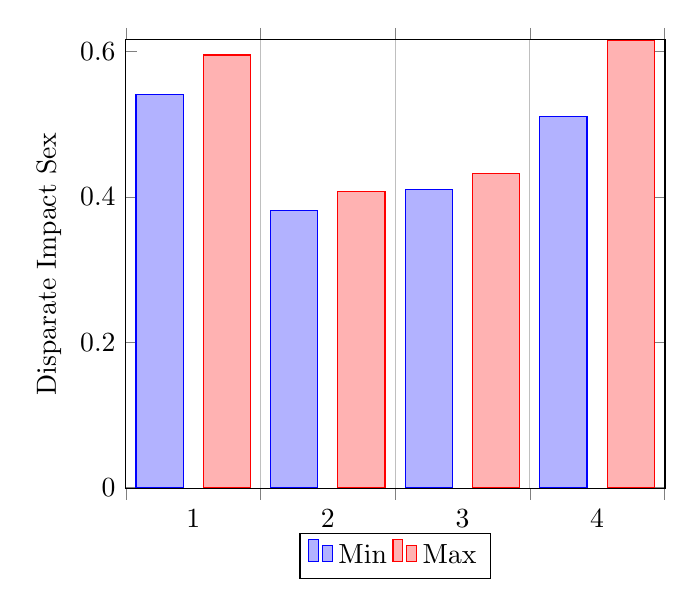
\begin{tikzpicture}
        \begin{axis}[
            x tick label style={
                /pgf/number format/1000 sep=},
            ylabel=Disparate Impact Sex,
            enlargelimits=0.001,
            legend style={at={(0.5,-0.1)},
            anchor=north,legend columns=-1},
            ybar interval=0.7,
        ]
        \addplot 
            coordinates {(1, 0.5409) (2, 0.3809) (3, 0.4103) (4, 0.5102) (5, 0.0000)};
        \addplot 
            coordinates {(1, 0.5950) (2, 0.4075) (3, 0.4325) (4, 0.6154) (5, 0.0000)};
        \legend{Min,Max}
        \end{axis}
        \end{tikzpicture}
    \caption{Min-Max Disparate Impact Metric for Sex protected attributes and for each fairness algorithm}
\end{figure}

The disparate impact metric measures the degree on which each algorithm reach the demographic parity for a certain protected attribute. In this scenario the \emph{Sex} protected attribute is considered and the following consideration can be made:

\begin{enumerate}
    \item \emph{Threshold Optimizer (TO) Demographic Parity Failure:} The Threshold Optimizer algorithm consistently fails to achieve demographic parity, as indicated by the perpetually zero values for this metric. This underscores the limitation of TO in addressing disparities associated with the \emph{Sex} attribute.

    \item \emph{Exponentiated Gradient (EG) Efficacy and Variability:} EG emerges as the algorithm that most effectively addresses demographic parity, showcasing the highest disparate impact values. However, it is also the algorithm with the maximum variance, indicating sensitivity to different experimental conditions.

    \item \emph{Grid Search (GS) Trade-off:} While GS demonstrates the minimum variance, it concurrently fails to achieve high values for demographic parity. This suggests a trade-off between stability and the ability to address demographic disparities in this context.

    \item \emph{Fairness Through Unawareness (FtU) Challenges:} Despite being the algorithm with the maximum accuracy, FtU fails to achieve demographic parity, highlighting potential challenges in its effectiveness for this specific fairness metric.

    \item \emph{Data Augmentation (DA) Performance:} DA, following EG, produces the highest values for disparate impact, indicating its efficacy in mitigating disparities associated with the \emph{Sex} attribute.

    \item \emph{Trade-off Consideration:} Assessing the trade-off between accuracy and the fairness metric, EG and DA emerge as promising candidates, showcasing a balance between achieving high accuracy and addressing demographic parity for the \emph{Sex} attribute.
\end{enumerate}

\paragraph{Disparate impact for race protected attribute}

\begin{figure}[H]
    \centering
    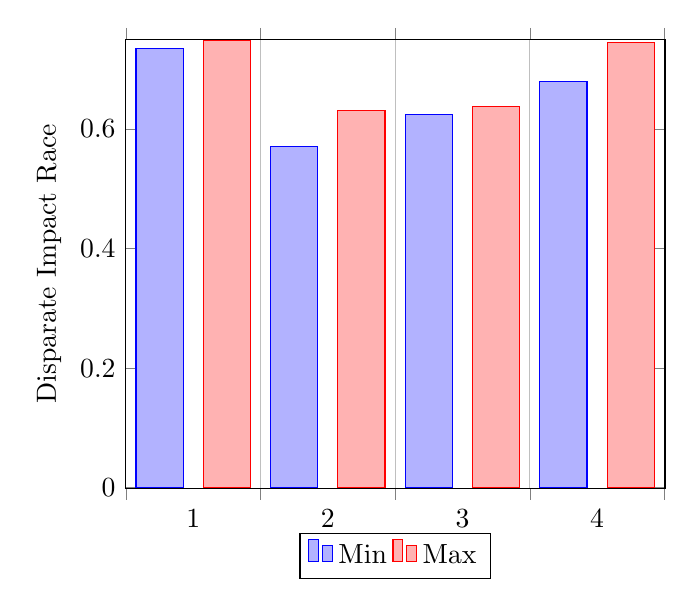
\begin{tikzpicture}
        \begin{axis}[
            x tick label style={
                /pgf/number format/1000 sep=},
            ylabel=Disparate Impact Race,
            enlargelimits=0.001,
            legend style={at={(0.5,-0.1)},
            anchor=north,legend columns=-1},
            ybar interval=0.7,
        ]
        \addplot 
            coordinates {(1, 0.7352) (2, 0.5703) (3, 0.6247) (4, 0.6802) (5, 0.0000)};
        \addplot 
            coordinates {(1, 0.7486) (2, 0.6308) (3, 0.6376) (4, 0.7442) (5, 0.0000)};
        \legend{Min,Max}
        \end{axis}
        \end{tikzpicture}
    \caption{Min-Max Disparate Impact Metric for Race protected attributes and for each fairness algorithm}
\end{figure}

Still considering the disparate impact metric but considering the \emph{Race} protected attribute it's possible to make the following considerations:

\begin{enumerate}
    \item \emph{Data Augmentation (DA) Performance:} DA not only provides the highest value for disparate impact but also exhibits minimal variance in its values. This makes DA a compelling choice as it effectively addresses disparities associated with the \emph{Race} attribute while maintaining stability.

    \item \emph{Threshold Optimizer (TO) Demographic Parity Failure:} Similar to the findings for the \emph{Sex} attribute, TO consistently fails to achieve demographic parity for the \emph{Race} attribute, underscoring its limitations in addressing disparities related to this protected attribute.

    \item \emph{Exponentiated Gradient (EG) Efficacy and Variability:} EG demonstrates high values for disparate impact, comparable to DA, but exhibits greater variance. Despite its efficacy, practitioners should be mindful of its sensitivity to different experimental conditions.

    \item \emph{Trade-off Consideration:} DA emerges as a standout performer, providing both the highest disparate impact values and minimal variance. This aligns with the trade-off requirements, making DA a strong candidate for practitioners seeking a balanced solution for the \emph{Race} attribute.
\end{enumerate}
\paragraph{Demographic parity difference for sex protected attribute}

\begin{figure}[H]
    \centering
    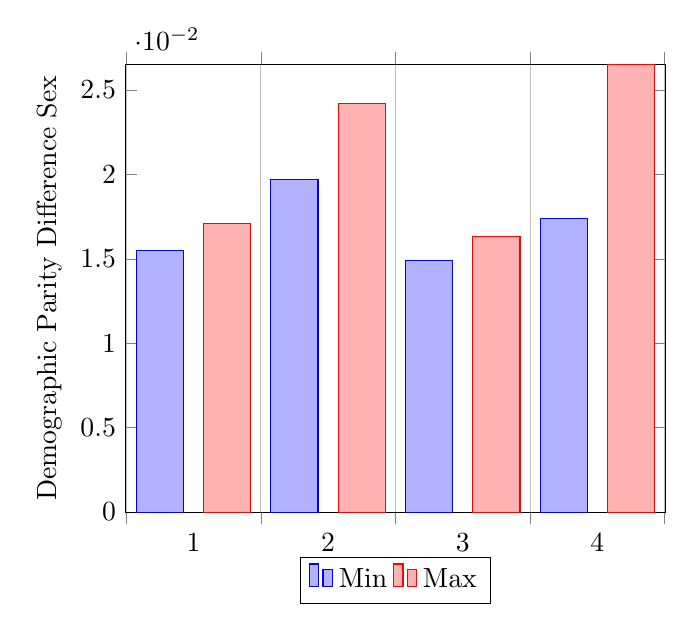
\begin{tikzpicture}
        \begin{axis}[
            x tick label style={
                /pgf/number format/1000 sep=},
            ylabel=Demographic Parity Difference Sex,
            enlargelimits=0.001,
            legend style={at={(0.5,-0.1)},
            anchor=north,legend columns=-1},
            ybar interval=0.7,
        ]
        \addplot 
            coordinates {(1, 0.0155) (2, 0.0197) (3, 0.0149) (4, 0.0174) (5, 0.0000)};
        \addplot 
            coordinates {(1, 0.0171) (2, 0.0242) (3, 0.0163) (4, 0.0265) (5, 0.0000)};
        \legend{Min,Max}
        \end{axis}
        \end{tikzpicture}
    \caption{Min-Max Demographic Parity Difference Metric for Sex protected attributes and for each fairness algorithm}
\end{figure}

The demographic parity difference metric measures the degree on which each algorithm reach the group fairness for a certain protected attribute. In this scenario the \emph{Sex} protected attribute is considered and the following consideration can be made:

\begin{enumerate}
    \item \emph{Exponentiated Gradient (EG) Dominance:} EG attains the maximum DPD value, indicating its success in achieving demographic parity. However, practitioners must consider the higher variance associated with these values, highlighting the algorithm's sensitivity to experimental conditions.

    \item \emph{Threshold Optimizer (TO) Group Fairness Achievement:} TO consistently provides the minimum DPD values, demonstrating its ability to perfectly achieve group fairness. Despite its lack of success in demographic parity, TO remains a strong contender for scenarios prioritizing group fairness.

    \item \emph{Data Augmentation (DA) and Grid Search (GS) Trade-off Consideration:} DA and GS exhibit comparable performances in terms of DPD. However, GS outperforms DA by a marginal accuracy improvement of 0.1\%. This nuanced trade-off consideration positions GS as a slightly more favorable choice, aligning with the objective of balancing accuracy and fairness.
\end{enumerate}

\paragraph{Demographic parity difference for race protected attribute}

\begin{figure}[H]
    \centering
    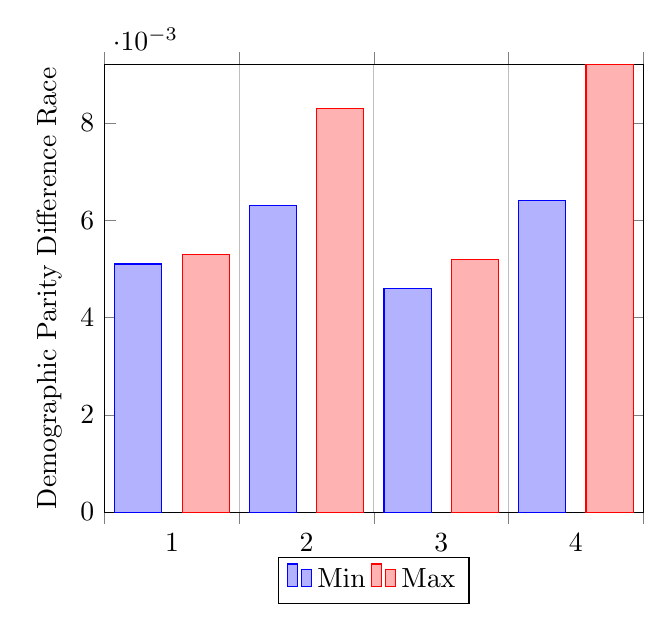
\begin{tikzpicture}
        \begin{axis}[
            x tick label style={
                /pgf/number format/1000 sep=},
            ylabel=Demographic Parity Difference Race,
            enlargelimits=0.001,
            legend style={at={(0.5,-0.1)},
            anchor=north,legend columns=-1},
            ybar interval=0.7,
        ]
        \addplot 
            coordinates {(1, 0.0051) (2, 0.0063) (3, 0.0046) (4, 0.0064) (5, 0.0000)};
        \addplot 
            coordinates {(1, 0.0053) (2, 0.0083) (3, 0.0052) (4, 0.0092) (5, 0.0000)};
        \legend{Min,Max}
        \end{axis}
        \end{tikzpicture}
    \caption{Min-Max Demographic Parity Difference for Race protected attributes and for each fairness algorithm}
\end{figure}

Still considering the demographic parity difference metric but considering the \emph{Race} protected attribute it's possible to make the following considerations:

\begin{enumerate}
    \item \emph{Threshold Optimizer (TO) Group Fairness Excellence:} TO consistently provides the minimum DPD values, showcasing its ability to achieve perfect group fairness. This makes TO an ideal choice for scenarios where group fairness is paramount.

    \item \emph{Exponentiated Gradient (EG) DPD Extremes:} EG attains the maximum DPD value, indicating its capability to maximize demographic parity. However, practitioners should be mindful of the higher variance associated with EG, suggesting sensitivity to experimental conditions.

    \item \emph{Data Augmentation (DA) and Grid Search (GS) Comparative Trade-off:} DA and GS exhibit comparable DPD values, with DA showcasing a slightly lower variance. This makes DA a potential selection when seeking a balanced trade-off between accuracy and fairness, with a preference for lower variance in DPD values.
\end{enumerate}


It's important to notice that every algorithm but Threshold Optimizer, which perfectly achieves the group fairness, for both the protected has values for the DPD that are very close to the 0. This means that the algorithms perform better achieving the Group Fairness than the Demographic Parity.